% Options for packages loaded elsewhere
\PassOptionsToPackage{unicode}{hyperref}
\PassOptionsToPackage{hyphens}{url}
%
\documentclass[
]{book}
\usepackage{amsmath,amssymb}
\usepackage{lmodern}
\usepackage{ifxetex,ifluatex}
\ifnum 0\ifxetex 1\fi\ifluatex 1\fi=0 % if pdftex
  \usepackage[T1]{fontenc}
  \usepackage[utf8]{inputenc}
  \usepackage{textcomp} % provide euro and other symbols
\else % if luatex or xetex
  \usepackage{unicode-math}
  \defaultfontfeatures{Scale=MatchLowercase}
  \defaultfontfeatures[\rmfamily]{Ligatures=TeX,Scale=1}
\fi
% Use upquote if available, for straight quotes in verbatim environments
\IfFileExists{upquote.sty}{\usepackage{upquote}}{}
\IfFileExists{microtype.sty}{% use microtype if available
  \usepackage[]{microtype}
  \UseMicrotypeSet[protrusion]{basicmath} % disable protrusion for tt fonts
}{}
\makeatletter
\@ifundefined{KOMAClassName}{% if non-KOMA class
  \IfFileExists{parskip.sty}{%
    \usepackage{parskip}
  }{% else
    \setlength{\parindent}{0pt}
    \setlength{\parskip}{6pt plus 2pt minus 1pt}}
}{% if KOMA class
  \KOMAoptions{parskip=half}}
\makeatother
\usepackage{xcolor}
\IfFileExists{xurl.sty}{\usepackage{xurl}}{} % add URL line breaks if available
\IfFileExists{bookmark.sty}{\usepackage{bookmark}}{\usepackage{hyperref}}
\hypersetup{
  pdftitle={An Introduction to Bayesian Statistics},
  pdfauthor={Manuele Leonelli},
  hidelinks,
  pdfcreator={LaTeX via pandoc}}
\urlstyle{same} % disable monospaced font for URLs
\usepackage{color}
\usepackage{fancyvrb}
\newcommand{\VerbBar}{|}
\newcommand{\VERB}{\Verb[commandchars=\\\{\}]}
\DefineVerbatimEnvironment{Highlighting}{Verbatim}{commandchars=\\\{\}}
% Add ',fontsize=\small' for more characters per line
\usepackage{framed}
\definecolor{shadecolor}{RGB}{248,248,248}
\newenvironment{Shaded}{\begin{snugshade}}{\end{snugshade}}
\newcommand{\AlertTok}[1]{\textcolor[rgb]{0.94,0.16,0.16}{#1}}
\newcommand{\AnnotationTok}[1]{\textcolor[rgb]{0.56,0.35,0.01}{\textbf{\textit{#1}}}}
\newcommand{\AttributeTok}[1]{\textcolor[rgb]{0.77,0.63,0.00}{#1}}
\newcommand{\BaseNTok}[1]{\textcolor[rgb]{0.00,0.00,0.81}{#1}}
\newcommand{\BuiltInTok}[1]{#1}
\newcommand{\CharTok}[1]{\textcolor[rgb]{0.31,0.60,0.02}{#1}}
\newcommand{\CommentTok}[1]{\textcolor[rgb]{0.56,0.35,0.01}{\textit{#1}}}
\newcommand{\CommentVarTok}[1]{\textcolor[rgb]{0.56,0.35,0.01}{\textbf{\textit{#1}}}}
\newcommand{\ConstantTok}[1]{\textcolor[rgb]{0.00,0.00,0.00}{#1}}
\newcommand{\ControlFlowTok}[1]{\textcolor[rgb]{0.13,0.29,0.53}{\textbf{#1}}}
\newcommand{\DataTypeTok}[1]{\textcolor[rgb]{0.13,0.29,0.53}{#1}}
\newcommand{\DecValTok}[1]{\textcolor[rgb]{0.00,0.00,0.81}{#1}}
\newcommand{\DocumentationTok}[1]{\textcolor[rgb]{0.56,0.35,0.01}{\textbf{\textit{#1}}}}
\newcommand{\ErrorTok}[1]{\textcolor[rgb]{0.64,0.00,0.00}{\textbf{#1}}}
\newcommand{\ExtensionTok}[1]{#1}
\newcommand{\FloatTok}[1]{\textcolor[rgb]{0.00,0.00,0.81}{#1}}
\newcommand{\FunctionTok}[1]{\textcolor[rgb]{0.00,0.00,0.00}{#1}}
\newcommand{\ImportTok}[1]{#1}
\newcommand{\InformationTok}[1]{\textcolor[rgb]{0.56,0.35,0.01}{\textbf{\textit{#1}}}}
\newcommand{\KeywordTok}[1]{\textcolor[rgb]{0.13,0.29,0.53}{\textbf{#1}}}
\newcommand{\NormalTok}[1]{#1}
\newcommand{\OperatorTok}[1]{\textcolor[rgb]{0.81,0.36,0.00}{\textbf{#1}}}
\newcommand{\OtherTok}[1]{\textcolor[rgb]{0.56,0.35,0.01}{#1}}
\newcommand{\PreprocessorTok}[1]{\textcolor[rgb]{0.56,0.35,0.01}{\textit{#1}}}
\newcommand{\RegionMarkerTok}[1]{#1}
\newcommand{\SpecialCharTok}[1]{\textcolor[rgb]{0.00,0.00,0.00}{#1}}
\newcommand{\SpecialStringTok}[1]{\textcolor[rgb]{0.31,0.60,0.02}{#1}}
\newcommand{\StringTok}[1]{\textcolor[rgb]{0.31,0.60,0.02}{#1}}
\newcommand{\VariableTok}[1]{\textcolor[rgb]{0.00,0.00,0.00}{#1}}
\newcommand{\VerbatimStringTok}[1]{\textcolor[rgb]{0.31,0.60,0.02}{#1}}
\newcommand{\WarningTok}[1]{\textcolor[rgb]{0.56,0.35,0.01}{\textbf{\textit{#1}}}}
\usepackage{longtable,booktabs,array}
\usepackage{calc} % for calculating minipage widths
% Correct order of tables after \paragraph or \subparagraph
\usepackage{etoolbox}
\makeatletter
\patchcmd\longtable{\par}{\if@noskipsec\mbox{}\fi\par}{}{}
\makeatother
% Allow footnotes in longtable head/foot
\IfFileExists{footnotehyper.sty}{\usepackage{footnotehyper}}{\usepackage{footnote}}
\makesavenoteenv{longtable}
\usepackage{graphicx}
\makeatletter
\def\maxwidth{\ifdim\Gin@nat@width>\linewidth\linewidth\else\Gin@nat@width\fi}
\def\maxheight{\ifdim\Gin@nat@height>\textheight\textheight\else\Gin@nat@height\fi}
\makeatother
% Scale images if necessary, so that they will not overflow the page
% margins by default, and it is still possible to overwrite the defaults
% using explicit options in \includegraphics[width, height, ...]{}
\setkeys{Gin}{width=\maxwidth,height=\maxheight,keepaspectratio}
% Set default figure placement to htbp
\makeatletter
\def\fps@figure{htbp}
\makeatother
\setlength{\emergencystretch}{3em} % prevent overfull lines
\providecommand{\tightlist}{%
  \setlength{\itemsep}{0pt}\setlength{\parskip}{0pt}}
\setcounter{secnumdepth}{5}
\usepackage{booktabs}
\ifluatex
  \usepackage{selnolig}  % disable illegal ligatures
\fi
\usepackage[]{natbib}
\bibliographystyle{apalike}

\title{An Introduction to Bayesian Statistics}
\author{Manuele Leonelli}
\date{2021-02-05}

\begin{document}
\maketitle

{
\setcounter{tocdepth}{1}
\tableofcontents
}
\hypertarget{preface}{%
\chapter*{Preface}\label{preface}}
\addcontentsline{toc}{chapter}{Preface}

These lecture notes are used to support the university course \emph{Bayesian Statistics} given to 3rd year students of the Bachelor in Data \& Business Administration at IE University, IE University, Madrid.

\hypertarget{intro}{%
\chapter{Introduction}\label{intro}}

Bayesian statistics is the name given to a whole branch of statistics which differs from the traditional approach taught in introductory statistics classes.

In order to understand what this difference is, let's first review the basic traditional approach, which is often referred to as \emph{frequentist} (we will see later on where this word comes from). In general, we are interested about an unknown characteristic of a population, usually called a population \emph{parameter}. For instance, we may be interested in the mean annual salary of an individual living in the city of Madrid. Let's call this quantity \(\mu\). Suppose it is impossible to exactly compute this quantity by accessing the information about the salary of everyone living in Madrid.

The next step would be to collect a sample, let's call it \(y\), with information about the salary of some inhabitants of Madrid. We would then use this sample to come up with a best guess, or an estimate, of \(\mu\). Due to multiple reasons which are not of interest here, we know that computing the sample mean \(\bar{y}\) is an optimal way to estimate \(\mu\) and we denote such a value \(\hat{\mu}\).

In most cases, having just a single value is not satisfactory enough, and we instead want an interval of values which would likely contain the true value \(\mu\). So a follow-up step would be to construct a so-called \emph{confidence interval}. You may recall that a confidence interval for a mean can be computed as
\[
\hat{\mu}\pm z_{\alpha}\sqrt{\frac{\hat{\sigma}^2}{n}},
\]
where

\begin{itemize}
\item
  \(n\) is the sample size;
\item
  \(\hat{\sigma}^2\) is an estimate of the population variance, that is a guess of how much variability there is around the mean;
\item
  \(z_{\alpha}\) is some value that comes either from a Normal or T-Student distribution which depends on how confident we want to be that the true \(\mu\) lies within the interval.
\end{itemize}

In the so-called frequentist approach we only used the data to guide the estimation of the unknown parameter and we assumed that we had no \emph{prior} information about what plausible values of \(\mu\) might be. Suppose on the other hand that in advance we had some guessing that the true value of \(\mu\) may lie within 20k and 50k. In the frequentist approach there is no way to embed this information within the inferential process. Only the data can be used to guide the estimation of the parameters. The \emph{Bayesian} approach on the other hand is designed to formally account prior information about the unknown parameter in the inferential process.

\hypertarget{a-more-technical-discussion}{%
\section{A more technical discussion}\label{a-more-technical-discussion}}

In order to understand how the Bayesian approach actually works, let's discuss slightly more formally how the frequentist estimation process works. Let's more generally call \(\theta\) the unknown population parameter that we want to estimate and \(y\) the sample. Depending on the type of data we are working with, we start choosing a statistical model, or a data-generating process, \(p(y|\theta)\). To make this clearer, consider the following examples:

\begin{itemize}
\item
  suppose that we observe coin tosses and we are interested in the probability of head: then the standard choice for \(p(y|\theta)\) would be the probability mass function of a Bernoulli distribution.
\item
  suppose we collect information about the number of goals scored in football matches: then the standard choice for \(p(y|\theta)\) would be the probability mass function of a Poisson distribution;
\item
  often we let \(p(y|\theta)\) be the probability density function of a Normal distribution. Such a choice is in general due to the \emph{Central Limit Theorem} which tells us that if our sample size is large enough then any distribution is well approximated by a Normal.
\end{itemize}

The quantity \(p(y|\theta)\) is also often referred to as the \emph{likelihood} and written as \(L(\theta|y)\). Notice that the order of \(\theta\) and \(y\) is reversed: whilst \(p(y|\theta)\) is seen as the distribution of \(y\) given the parameter \(\theta\), \(L(\theta|y)\) is seen as a measure of how likely is that the parameter is \(\theta\) given that we observed the sample \(y\).

No matter what the interpretation is, we view as random only the process that generated the data which is assumed to behave according to some distribution \(p(y|\theta)\). The parameter \(\theta\) is itself assumed to be fixed and unknown: it is not random, it is just that we do not know its value. We use \(p(y|\theta)\) to come up with an estimate \(\hat\theta\) of the unknwon \(\theta\). For instance in maximum likelihood estimation \(\hat\theta\) is found as
\[
\hat\theta = \arg\max_{\theta} p(y|\theta)
\]

The Bayesian approach differs from the frequentist approach since it consider the unknown parameter \(\theta\) to also be a random variable and not simply fixed. Therefore in Bayesian statistics the unknown parameter is also assigned a distribution, \(p(\theta)\), which is referred to as \emph{prior} distribution. Furthermore, the main building block of Bayesian statistics is a joint distribution for the data-generating process and the unknown parameter, since both are random. Such a distribution is
\[
p(y,\theta),
\]
which by using basic rules of conditional probabilities can be written as
\[
p(y,\theta) = p(y|\theta)p(\theta).
\]
The above expression can be seen as the product of the data-generating distribution, or likelihood, with the prior distribution.

The prior distribution encodes our beliefs about the unknown parameter of interest before observing any data. Now suppose we collect the sample \(y\): we would like to use it to revise or update our beliefs about the unknown parameter \(\theta\). This is done using Bayes theorem, hence the name Bayesian statistics. Most likely, you are already familiar with the version of Bayes theorem for events namely:
\[
P(A|B) = \frac{P(B|A)P(A)}{P(B)}.
\]
Similarly we can write

\begin{equation}
 \label{eq:posterior}
p(\theta|y) = \frac{p(y|\theta)p(\theta)}{p(y)}
\end{equation}

and \(p(\theta|y)\) is usually called the \emph{posterior distribution}: it encodes our beliefs about \(\theta\) after having observed the sample \(y\). Equation \eqref{eq:posterior} is the backbone of Bayesian statistics and the main task in a Bayesian analysis is to compute such a posterior distribution.

There are two important observations to make now. First, in Equation \eqref{eq:posterior} the terms \(p(y|\theta)\) and \(p(\theta)\) are chosen by the modeler, whilst \(p(y)\) can be computed from these two as:
\[
p(y)=\int p(y,\theta)d\theta=\int p(y|\theta)p(\theta)d\theta
\]
and it is called \emph{marginal likelihood}. So Equation \eqref{eq:posterior} can also be written as
\[
p(\theta|y) = \frac{p(y|\theta)p(\theta)}{\int p(y|\theta)p(\theta)d\theta}.
\]

Second, our object of study is the parameter \(\theta\) and \(p(\theta|y)\) is a function of \(\theta\) only. So the term \(p(y)\) at the denominator of Equation \eqref{eq:posterior} is actually only a normalization constant to make sure that \(p(\theta|y)\) integrates to 1. So Equation \eqref{eq:posterior} is often presented as

\begin{equation}
 \label{eq:posterior1}
p(\theta|y)\propto p(y|\theta)p(\theta).
\end{equation}

Equation \eqref{eq:posterior1} is actually the one that most often we will work with since \(p(y)\) is not actually necessary and it is often very hard to compute.

One question you might have is: why did we combine the prior distribution and data-generating distribution using Bayes Theorem? We could have used different rules to come up with a so-called posterior distribution. We will not enter into the details of this, but if beliefs are encoded as probability distributions, then it can proved that Bayes theorem is the optimal way to update them in the light of data.

\hypertarget{a-first-example}{%
\section{A first example}\label{a-first-example}}

Suppose we are interested in estimating the prevalence of COVID-19 cases in the city of Madrid. For this purpose we select a sample of 100 individuals living in the city. Let's assume that each individual has the same probability of having the disease and that each individual has the disease independently of others.

Then we could model the fact that each individual has the disease as a Bernoulli distribution, where the value 1 denotes having the disease. Suppose the result of COVID testing over these 100 individuals shows that 10 of them are positive. Then we would estimate the parameter \(\theta\) of the Bernoulli distribution as \(\hat\theta=10/100=0.1\), which would in turn be our estimate for the prevalence of COVID cases in Madrid. Furthermore, we could construct a 95\% confidence interval which, if you recall from previous courses, can be computed as
\[
\hat\theta\pm 1.96 \sqrt{\frac{\hat\theta(1-\hat\theta)}{n}}= 0.1 \pm 1.96 \sqrt{\frac{0.1\cdot 0.9}{100}}= (0.041,0.159).
\]

Let's take a Bayesian approach instead. For the data-generating process it is still of course reasonable to believe that a Bernoulli distribution with unknown parameter \(\theta\) is appropriate. Now we also need to define a prior distribution. Suppose that from data related to other European cities, we believe that such a prevalence number is between 0.05 and 0.25 with an average around 0.15. We will later learn ways to choose prior distributions, but suppose that such a prior information can be represented by the distribution colored in blue in Figure \ref{fig:example}. This distribution represents our beliefs about the prevalence of COVID in the city of Madrid.

\begin{figure}
\centering
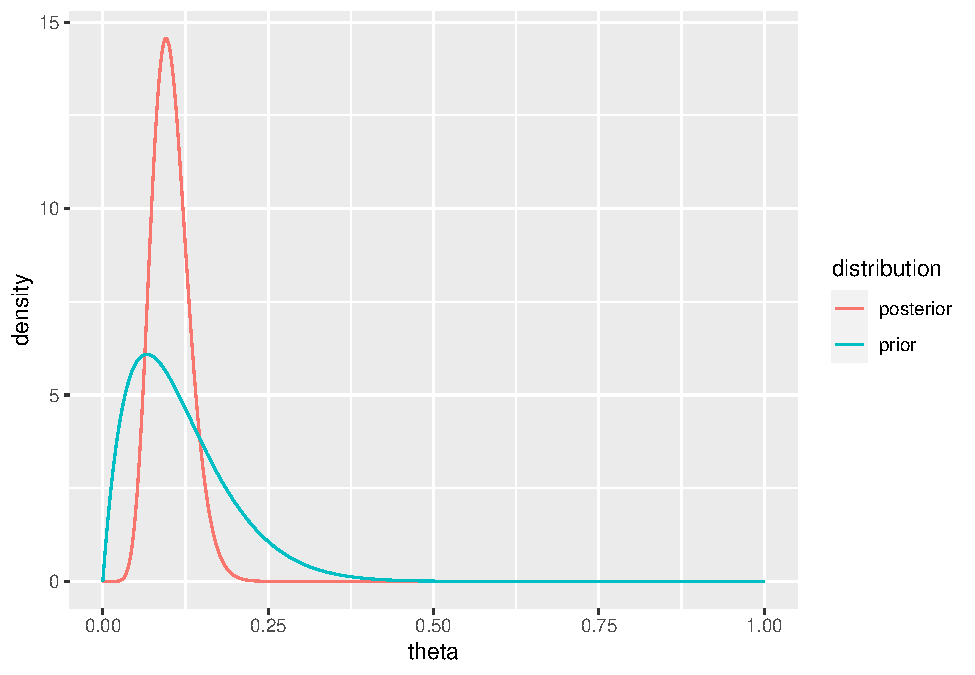
\includegraphics{BayesStats_files/figure-latex/example-1.pdf}
\caption{\label{fig:example}Prior and posterior distribution for the COVID example.}
\end{figure}

Suppose we collect the same sample as before of 10 positive out of 100 and compute the posterior distribution using Bayes theorem. This is reported in Figure \ref{fig:example} by the red distribution. So differently from the frequentist case where we have a single point estimate of \(\theta\) or a confidence interval of plausible values, we now have a full distribution for the variable \(\theta\) in the light of data and prior beliefs. Given such a distribution we can do multiple things:

\begin{itemize}
\item
  we can come up with a single point estimate for \(\theta\), for instance the mean or the mode of the distribution;
\item
  we can identify a plausible region of values of \(\theta\) in the same spirit of a confidence interval.
\end{itemize}

It is important to notice that our beliefs about the prevalence of COVID has now changed in the light of data. Our prior distribution was quite spread around values between 0.05 and 0.25, whilst the posterior is a lot more concentrated around 0.1 which is actually the sample proportion of COVID.

\hypertarget{why-bayesian-statistics}{%
\section{Why Bayesian statistics}\label{why-bayesian-statistics}}

The previous example showed an example of a simple Bayesian analysis and how it differs from a frequentist one. One might wonder what is the real advantage of taking a Bayesian approach with respect to a frequentist one: we saw that in the end the conclusion from both approaches was pretty much the same.

In general we can notice the below advantages of a Bayesian approach:

\begin{itemize}
\item
  it allows to more flexibly construct complicated models. This is a concept we will see in later chapters when we will discuss hierarchical models;
\item
  it allows to easily embed in inference other type of information which is not only in the form of data: for instance, expert judgment or results from other studies;
\item
  it allows to use data in a sequential manner. Suppose we carried out our analysis about COVID prevalence and once finished we are actually given the result of tests on new individuals. In the Bayesian framework, we could then use our posterior from the previous step as our new prior and use the same machinery to come up with a new posterior. In a frequentist setting, we would need to use the full dataset again to come up with an estimate of \(\theta\). Of course this is trivial in the COVID example, but for much more complicated models, it may be very costly to repeat the analysis with the full dataset.
\item
  it leads to an intuitive interpretation of confidence intervals. Standard confidence intervals are probability statements about \(\hat\theta\) and not \(\theta\) itself as often erraneosly thought. The correct interpretation of a 95\% confidence interval is that if we were to collect many many times samples under the same conditions and each time construct a confidence interval, then 95\% of the times the interval would include the true value \(\theta\). However, most often people interpret confidence intervals as with 95\% probability the true unknown parameter lies in the interval, which is not correct. However, this is the interpretation of confidence intervals in the Bayesian setup;
\item
  it can deal more easily with rare situations. Let's consider the COVID example again and suppose that on the other hand we observed zero positive tests. Then our point estimate of the prevalance would be zero and confidence intervals at any level of confidence (even 99.9999\%) would simply be the point zero, which we would in general not believe unless the sample size is extremely large! Using the same prior as before, in the case of zero positive cases our posterior would be the one in Figure \ref{fig:example1}. Although most of the distribution is around zero, we still have some probability that the prevalence is some small number close to zero. The more and more only negative tests we would collect, the more the distribution would be concentrated in zero!
\end{itemize}

\begin{figure}
\centering
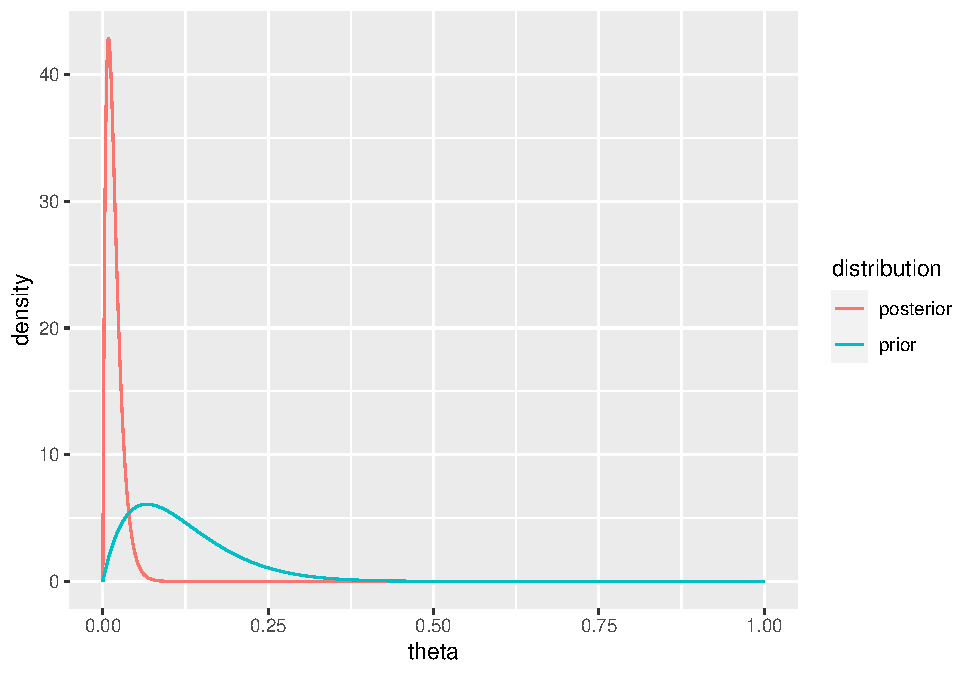
\includegraphics{BayesStats_files/figure-latex/example1-1.pdf}
\caption{\label{fig:example1}Prior and posterior distribution for the COVID example.}
\end{figure}

Of course there are also drawbacks of the Bayesian approach. The main critic regards the prior distribution and the addition of a ``subjective'' element in the analysis. We will discuss a lot more this issue in the next chapter. The second drawback is that it is computationally much more expensive and most often Bayesian methods require more computational power and computational time. As we will see in the next section, this was actually one of the reasons Bayesian methods were not used for many years.

\hypertarget{a-bit-of-history}{%
\section{A bit of history}\label{a-bit-of-history}}

The term Bayesian statistics comes from the fact that inference is based upon a sequential use of Bayes theorem. Reverend Thomas Bayes was an English minister whose 1763 posthumosly paper ``An Essay Towards Solving a Problem in the Doctrine of Chances'' gives the first account of what we now call Bayes theorem. As a matter of fact, his account of the result is not in the form you are familiar with. It was Pierre Simon Laplace, an 18th century French scientist, who introduced Bayes theorem in a form much more similar to the one we use today in his essay ``Memoire sur la Probabilite des Causes par les Evenements''.

Laplace was actually studying the probability of a ``success'' in a Binomial experiment given that data was observed. In the terminology we introduced he was characterizing the posterior distribution of \(\theta\). The method of deriving a probability distribution for an unknown parameter given data was overall called the ``inverse probability'' problem and became the gold standard throughout the 19th century.

Of course there were many scientists that critiqued such a method, including Boole and Venn, due to the non-objectivity of the method. However, since no alternative was available at the time, the inverse probability method continued to be the gold-standard.

It was only at the beginning of the 20th century with the work of Ronald Alymer Fisher, Jerzy Neyman and Egon Pearson, that the frequentist approach became to emerge. Therefore, the approach of statistics that is most frequently taught is actually less recent than Bayesian ideas.

Although frequentist approached dominated statistics, Bayesian ideas were still being developed in the first half of the 20th century through the work on subjective probabilities of Harold Jeffreys, Bruno de Finetti and Leonard Savage.

In the second half of the century there was a resurgence of Bayesian methods. Two of the main reasons were:

\begin{itemize}
\item
  the work on expected utility of von Neumann and Morgenstern where a subjective view of probability can be more easily accepted became very popular;
\item
  computational power increased at a speed never seen before and a lot of complex problems could be at last approached with a Bayesian approach.
\end{itemize}

Nowadays Bayesian statistics is as popular as frequentist statistics and research is carried out almost equally in the two frameworks. There are indeed problems that can be more easily tackled with a Bayesian approach (and the other way around too, of course!).

\hypertarget{interpretations-of-probability}{%
\section{Interpretations of probability}\label{interpretations-of-probability}}

The field of Bayesian statistics is deeply connected to a different interpretation of probability then the ones you are probably familiar with.

The most common and basic interpretation of probability is due to Pierre Simon Laplace and is based on the notion of symmetry of elementary outcomes or, to put it differently, on the notion of equiprobability. In Laplace's definition the probability of an event is defined as the number of favourable cases over the number of total cases. Let's consider the throw of a simple dice and the event that the number shown is even. There are three favourable cases (2,4 and 6) and six total cases (the numbers from 1 to 6). The probability of this event is therefore one half as one would expect. Of course this definition applies only to cases where elementary outcomes are equiprobable: in the example if the dice is not biased.

The second most common interpretation is the so-called \emph{frequentist} one. Probability is defined as the relative frequency in a long sequence of identical independent trials. It is assumed that there is an underlying generating process which every times generates an independent instance. Let's consider again the event of an even number in a dice throw. The probability of this event is defined as the frequency of even numbers if we were to repeat the throw of a dice an infinite number of times. Figure \ref{fig:dice} illustrates how the relative frequency of even numbers evolves in 500 throws. The red line is the relative frequency: for the first 100 tries it is quite far away from the value 0.5 and then it slowly stabilizes at the true value.

\begin{Shaded}
\begin{Highlighting}[]
\FunctionTok{set.seed}\NormalTok{(}\DecValTok{2021}\NormalTok{)}
\NormalTok{x }\OtherTok{\textless{}{-}} \FunctionTok{sample}\NormalTok{(}\DecValTok{1}\SpecialCharTok{:}\DecValTok{6}\NormalTok{,}\DecValTok{500}\NormalTok{,}\ConstantTok{TRUE}\NormalTok{)}\SpecialCharTok{\%\%} \DecValTok{2} \SpecialCharTok{==} \DecValTok{0}
\FunctionTok{plot}\NormalTok{(}\FunctionTok{cumsum}\NormalTok{(x)}\SpecialCharTok{/}\DecValTok{1}\SpecialCharTok{:}\DecValTok{500}\NormalTok{,}\AttributeTok{type=}\StringTok{"l"}\NormalTok{, }\AttributeTok{ylim =} \FunctionTok{c}\NormalTok{(}\DecValTok{0}\NormalTok{,}\DecValTok{1}\NormalTok{), }\AttributeTok{col =} \StringTok{"red"}\NormalTok{, }\AttributeTok{ylab=}\StringTok{"Probability"}\NormalTok{)}
\FunctionTok{abline}\NormalTok{(}\AttributeTok{h=}\FloatTok{0.5}\NormalTok{)}
\end{Highlighting}
\end{Shaded}

\begin{figure}

{\centering 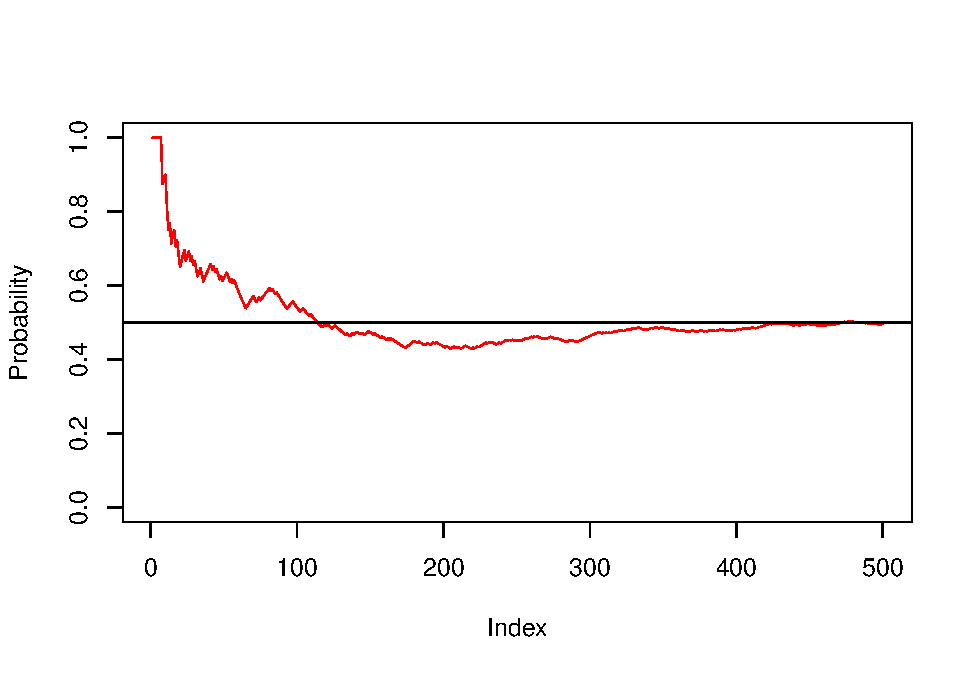
\includegraphics[width=0.5\linewidth]{BayesStats_files/figure-latex/dice-1} 

}

\caption{Relative frequency of even numbers in 500 dice throws}\label{fig:dice}
\end{figure}

Now let's think at some other types of events:

\begin{itemize}
\item
  Spain winning the next world cup;
\item
  the next expedition to Mars fails;
\item
  it rains tomorrow.
\end{itemize}

It becomes challenging to define probability as relative frequency since we cannot think of a sequence of repetitions of such processes that are exactly equal. Such events are in general \emph{non-reproducible}. However, we can think of defining a probability that these events happen, which in a way encodes our \emph{degree of belief} that the event will happen. Notice that such a degree of belief is personal and may vary from individual to individual (a Spaniard may give a higher probability of Spain winning a World Cup than a foreigner). For this reason, this interpretation of probability is usually referred to as \emph{subjective}.

A classical way to define probabilities in the subjective framework is in terms of betting odds. Consider an event \(A\). Then \(P(A)\), the probability of \(A\), is the amount you are willing to pay for a lottery ticket that pays one Euro if \(A\) happens. Notice the \emph{you} in the previous sentence. It is your probability and depends on the information available to \emph{you}. We will not focus on this, but it has been proved that if one specifies probabilities in this way, and assuming you choose the numbers in order to win money, then subjective probabilities respect the usual axioms probabilities (probabilities are numerical quantities, defined
on a set of `outcomes,' that are non-negative, additive over mutually exclusive outcomes, and sum to 1 over all possible mutually exclusive outcomes).

The following quote from De Finetti is provocative.

\begin{quote}
My thesis, paradoxically, and a little provocatively, but nonetheless
genuinely, is simply this:

PROBABILITY DOES NOT EXIST

The abandonment of superstitious beliefs about the existence of Phlogiston, the Cosmic Ether, Absolute Space and Time, . . . , orFairies and Witches, was an essential step along the road to scientific thinking. Probability, too, if regarded as something endowed with some kind of objective existence, is no less a misleading misconception, an illusory attempt to exteriorize or materialize our true probabilistic beliefs.
\end{quote}

This interpretation of probability is the one underlying most Bayesian analyses. In Bayesian statistics unknown quantities (for instance parameters of interest) are random variables and probabilities must be assigned to them by the modeler.

Another approach sees probability as a \emph{logic of plausibility}. This approach was put forward by statisticians as Jeffreys, Cox and Jaynes. According to this interpretation, the rules of probability extend ordinary (``Boolean'') logic, where statements are known to be either true or false, to inductive logic, where statements are true or false, but we don't know which. Probability is then a scale used to describe how strongly, based on specific information, we believe a statement to be true. It is a more objective approach in the sense that anyone with the same knowledge should assign the same probabilities. Again we will not focus on this, but then one can prove the probabilities so defined obey the usual axioms.

The following quote from Maxwell gives a justification of this approach.

\begin{quote}
They say that Understanding ought to work by the rules of right reason. These rules are, or ought to be, contained in Logic; but the actual science of logic is conversant at present only with things either certain, impossible, or entirely doubtful, none of which (fortunately) we have to reason on. Therefore the true logic for this world is the calculus of Probabilities, which takes account of the magnitude of the probability which is, or ought to be, in a reasonable man's mind.
\end{quote}

The above discussion is brief and not at all comprehensive but it should have given you at least an idea of possible different interpretations of probability.

\hypertarget{a-review-of-probability}{%
\section{A review of probability}\label{a-review-of-probability}}

\hypertarget{random-variables}{%
\subsection{Random variables}\label{random-variables}}

A random variable is defined as an unknown numerical quantity about which we make probability statements.

\hypertarget{discrete-random-variables}{%
\subsubsection{Discrete random variables}\label{discrete-random-variables}}

Let \(Y\) be a random variable and \(\mathbb{Y}\) be the set of all possible values of \(Y\). Usually, \(\mathbb{Y}\) is called the \emph{sample space}. We say that \(Y\) is discrete if \(\mathbb{Y}\) is countable, meaning that \(\mathbb{Y}\) can be expressed as \(\mathbb{Y} = \{y_1, y_2,\dots\}\).

For each \(y\in\mathbb{Y}\), we define the \emph{probability density function} (pdf) \(p(y)=P(Y=y)\) which must obey the following conditions:

\begin{itemize}
\item
  \(p(y)\geq 0\) for all \(y\in\mathbb{Y}\);
\item
  \(\sum_{y\in\mathbb{Y}}p(y)=1\).
\end{itemize}

For any \(A\subseteq \mathbb{Y}\), the probability that \(Y\in A\) can be computed via summation as
\[
P(Y\in A) = \sum_{y\in A} p(y).
\]

\hypertarget{continuous-random-variables}{%
\subsubsection{Continuous random variables}\label{continuous-random-variables}}

If the sample space \(\mathbb{Y}\) is an interval, not necessarily finite (for instance it could be the set of all real numbers \(\mathbb{R}\)), we say that \(Y\) is a continuous random variable.

The pdf of a continuous random variable \(Y\) is now defined as the function \(p\) for which:
\[
P(a\leq Y \leq b) = \int_a^b p(y)dy
\]

We cannot define \(P(a \leq Y \leq b)\) as equal to \(\sum_{a\leq y \leq b}p(y)\) because the sum does not make sense (the set of real numbers between \(a\) and \(b\) is ``uncountable''). So pdfs are defined indirectly as the function such that its integral is the probability of the corresponding event.

The pdf of a continuous random variable must again obey two conditions:

\begin{itemize}
\item
  \(p(y)\geq 0\), for all \(y\in\mathbb{Y}\);
\item
  \(\int_{y\in\mathbb{R}}p(y)dy =1\).
\end{itemize}

We can see that integration for continuous distributions behaves similarly to summation for discrete distributions. In fact, integration can be thought of as a generalization of summation for situations in which the sample space is not countable. However, unlike a pdf in the discrete case, the pdf for a continuous
random variable is:

\begin{itemize}
\item
  Not necessarily less than 1;
\item
  \(p(y)\) is not ``the probability that \(Y = y\)'';
\item
  such that \(P(Y=y)=0\) for any \(y\in\mathbb{Y}\).
\end{itemize}

However, if \(p(y_1) > p(y_2)\) we will sometimes informally say that \(y_1\) ``has a higher probability'' than \(y_2\).

\hypertarget{joint-distributions}{%
\subsection{Joint distributions}\label{joint-distributions}}

\hypertarget{discrete-case}{%
\subsubsection{Discrete case}\label{discrete-case}}

Let \(Y_1\) and \(Y_2\) be two discrete random variables with \(\mathbb{Y}_1\) and \(\mathbb{Y}_2\) as sample spaces, respectively. We are often interested in joint beliefs about two variables. For instance we may want to know
\[
P(Y_1=y_1,Y_2=y_2), \hspace{1cm} \mbox{for } y_1\in\mathbb{Y}_1 \mbox{ and } y_2\in \mathbb{Y}_2
\]

The (joint) pdf is then \(p(y_1,y_2)=P(Y_1=y_1,Y_2=y_2)\).

The \emph{marginal density} of \(Y_1\) can be computed from the joint as:
\[
p(y_1)=P(Y_1=y_1)=\sum_{y_2\in\mathbb{Y}_2}P(Y_1=y_1,Y_2=y_2)=\sum_{y_2\in\mathbb{Y}_2}p(y_1,y_2)
\]

The \emph{conditional density} of \(Y_2\) given \(Y_1=y_1\) can be computed from the joint and the marginal as:
\[
p(y_2|Y_1=y_1)=\frac{p(y_1,y_2)}{p(y_1)}
\]
Re-arranging the above equation we can also see that
\[
p(y_1,y_2)= p(y_2|Y_1=y_1)p(y_1)
\]

Let's consider an example. Suppose we have a random variable \(Y_1\) which is the outcome of a COVID-19 test (either positive or negative) and \(Y_2\) which is whether an individual has COVID or not (sick or healthy). The joint probability distribution is defined as

\[
\begin{matrix}
    \begin{array}{c|cc} \hline
    &\text{sick} & \text{healthy} \\\hline
    \text{positive} & 0.10 & 0.09 \\\hline
    \text{negative} & 0.01 & 0.80 \\\hline
    \end{array}
\end{matrix}
\]

The above table is a joint pdf since all numbers are positive and sum to one. The marginal probability of \(Y_1\) (test result) is the row sums: 19\% of tests are positive and 81\% of tests are negative. The marginal probability of \(Y_2\) is the column sums: 11\% of individuals are sick and 89\% are healthy. Given these marginals we can also compute conditional probabilities:

\begin{itemize}
\item
  \(p(\text{positive}|\text{sick})= \frac{p(\text{positive},\text{sick})}{p(\text{sick})}=\frac{0.10}{0.11}=0.91\)
\item
  therefore \(p(\text{negative}|\text{sick})=0.09\).
\end{itemize}

Other conditional probabilities can be derived similarly.

\hypertarget{continuous-case}{%
\subsubsection{Continuous case}\label{continuous-case}}

In the continuous case the definitions are analogous but summations are substituted with integrals. For instance,
\[
p(y_1)= \int_{y_2\in\mathbb{Y}_2}p(y_1,y_2)dy_2
\]

\hypertarget{expectation-and-variance}{%
\subsection{Expectation and variance}\label{expectation-and-variance}}

The mean or expectation of a random variable \(Y\) is

\begin{itemize}
\item
  \(E(Y)=\sum_{y\in\mathbb{Y}} y p(y)\) in the discrete case;
\item
  \(E(Y)=\int_{y\in\mathbb{Y}}yp(y)dy\) in the continuous case.
\end{itemize}

The mean is the center of mass of the distribution.

In addition to the location of a distribution we are often interested in how
spread out it is. The most popular measure of spread is the variance of a
distribution:
\[
V(Y)=E((Y-E(Y))^2)= E(Y^2) - E(Y)^2
\]
The variance is the average squared distance between values of \(Y\) and its mean \(E(Y)\). The standard deviation is the square root of the variance, and is on the same scale as \(Y\).

Above we have defined conditional densities of the form \(p(y_2|Y_1=y_1)\). Since formally they are pdfs they have expectation and variance which are usually denoted as \(E(Y_2|Y_1=y_1)\) and \(V(Y_2|Y_1=y_1)\).

Furthermore, it is often useful to express the mean and variance of a random variable \(Y_2\) in terms of the conditional mean and variance given some related quantity \(Y_1\). The mean of \(Y_2\) can be obtained by averaging the conditional mean over the marginal distribution of \(Y_1\):
\[
E(Y_2)=E(E(Y_2|Y_1=y_1)).
\]
Let's see why this is true:
\begin{eqnarray*}
E(Y_2) &=&\sum_{y_2\in\mathbb{Y}_2}y_2p(y_2)\\
 &=&\sum_{y_2\in\mathbb{Y}_2}y_2\sum_{y_1\in\mathbb{Y}_1}p(y_1,y_2)\\
 &=&\sum_{y_2\in\mathbb{Y}_2}\sum_{y_1\in\mathbb{Y}_1}y_2p(y_2|Y_1=y_1)p(y_1)\\
 &=&\sum_{y_1\in\mathbb{Y}_1}p(y_1)\sum_{y_2\in\mathbb{Y}_2}y_2p(y_2|Y_1=y_1)\\
 &=&\sum_{y_1\in\mathbb{Y}_1}p(y_1)E(Y_2|Y_1=y_1)\\
 &=& E(E(Y_2|Y_1=y_1))
\end{eqnarray*}

The corresponding result for the variance includes two terms, the mean of the conditional
variance and the variance of the conditional mean:
\[
V(Y_2) = E(V(Y_2|Y_1=y_1)) + V(E(Y_2|Y_1=y_1))
\]

\hypertarget{independence}{%
\subsection{Independence}\label{independence}}

We say that two random variables are independent if
\[
p(y_1,y_2) = p(y_1)p(y_2)
\]
that is if the joint distribution can be written as the product of the marginal distributions.

In Bayesian statistics we usually make the assumption that we have independent random variables \(Y_1,Y_2,\dots,Y_N\) which all depend on a parameter \(\theta\), which is also believed to be random variable. We say that \(Y_1,\dots,Y_N\) are conditionally independent given \(\theta\) if
\[
p(y_1,\dots,y_N|\theta)=\prod_{i=1}^Np(y_i|\theta).
\]
Another way to say this is that \(Y_1,\dots,Y_N\) are conditionally independent and identically distributed (iid).

Notice that in standard statistical practice when we analyze a sample we start with the assumption that the data are realizations of independent and identically distributed random variables (not conditionally, since the parameter is not considered random).

\hypertarget{exchangeability}{%
\section{Exchangeability}\label{exchangeability}}

In many situations with several random variables, we would believe that the specific order of observation of these random variables is not important. For example, consider a random sample of 3 participants from an infinite population which may or may not have a property (1 or 0) It makes sense that
\[
p(1,0,0) = p(0,1,0) = p(0,0,1).
\]
Such a property is called \emph{exchangeability}.

Let \(Y_1,\dots,Y_N\) be random variables. If \(p(y_1,\dots,y_N)=p(y_{\pi_1},\dots,y_{\pi_N})\) for all permutations \(\pi\) of \(\{1,\dots,N\}\), then \(Y_1,\dots,Y_N\) are exchangeable.

Roughly speaking, \(Y_1,\dots, Y_n\) are exchangeable if the subscript labels convey no information about the outcomes.

The following result (often called De Finetti's Theorem) tells us that it is sufficient to assume exchangeability for random variables to be (conditionally) iid.

\[
Y_1,\dots,Y_N \mbox{ are iid } \Longleftrightarrow Y_1,\dots,Y_n \mbox{ are exchangeable for all N's}
\]

So notice that in Bayesian statistics we are actually starting from a weaker assumption about the data-generating process.

\hypertarget{whats-next}{%
\section{What's next}\label{whats-next}}

This introduction should have given you a feeling of what a Bayesian analysis entails and the various steps required. In the next chapters we will dig deeper into the various components of a Bayesian analysis, namely:

\begin{itemize}
\item
  we will learn how to compute posterior distributions for a variety of simple models;
\item
  we will discuss how to summarize a posterior distribution to come up with point estimates and confidence intervals;
\item
  we will investigate various types of prior distributions and their effect to the posterior distribution;
\item
  we will learn how to construct more complex models within a Bayesian framework, which are usually called hierarchical or multilevel models.
\end{itemize}

  \bibliography{book.bib,packages.bib}

\end{document}
